% ════════════════════════════════════════════════════════════════
\subsection{Problem sumy podzbioru} \label{subsec:subsetsum-cd}
% ════════════════════════════════════════════════════════════════

Kontynuujemy analizę w~pełni wielomianowego schematu aproksymacyjnego dla problemu sumy podzbiorów (Problem~\ref{problem:subsetsum}). Przypomnijmy schemat \Call{ApproxSubsetSum}{} (Algorytm~\ref{alg:approxsubsetsum}) wraz z~procedurą \Call{Trim}{} (Algorytm~\ref{alg:trim}); ustalamy $\delta = \frac{\epsilon}{2n}$. Pokażemy najpierw przykład jego działania, a~następnie dowód poprawności i~analizę złożoności.

\begin{example}[Aproksymacja sumy podzbioru]
	$S = \{205, 203, 400, 200\}$ (w~tej kolejności $x_1, \ldots, x_4$), $t = 650$, $\varepsilon = 0{,}4$. Wtedy $n = 4$ i~próg przycinania to $\delta = \frac{\varepsilon}{2n} = \frac{0{,}4}{8} = 0{,}05$ (mnożnik $1 + \delta = 1{,}05$). Startujemy z~$L_0 = (0)$.

	W~każdej iteracji najpierw scalamy $L_{i-1}$ z~$L_{i-1} + x_i$, potem usuwamy elementy $> t = 650$, a~na końcu przycinamy. Przy przycinaniu zachowujemy element $y$, gdy $y > last \cdot 1{,}05$, gdzie $last$ to ostatnio zachowany element.
	\begin{itemize}[nosep]
		\item \textbf{$i = 1$, $x_1 = 205$.} \\
		      scalenie: $(0) \cup (205) = (0, 205)$; \\
		      po usunięciu $> 650$: $(0, 205)$; \\
		      przycinanie: \\
		      \begin{tblr}{colspec={r c l l}, column{4}={font=\itshape}, rowsep=1pt}
			      $0$   &     &                     & zachowane, $last = 0$   \\
			      $205$ & $>$ & $0 \cdot 1{,}05 = 0$ & zachowane, $last = 205$ \\
		      \end{tblr} \\
		      $L_1 = (0, 205)$.
		\item \textbf{$i = 2$, $x_2 = 203$.} \\
		      scalenie: $(0, 205) \cup (203, 408) = (0, 203, 205, 408)$; \\
		      po usunięciu $> 650$: bez zmian; \\
		      przycinanie: \\
		      \begin{tblr}{colspec={r c l l}, column{4}={font=\itshape}, rowsep=1pt}
			      $0$   &        &                               & zachowane, $last = 0$   \\
			      $203$ & $>$    & $0$                           & zachowane, $last = 203$ \\
			      $205$ & $\leq$ & $203 \cdot 1{,}05 = 213{,}15$ & usunięte                \\
			      $408$ & $>$    & $213{,}15$                    & zachowane, $last = 408$ \\
		      \end{tblr} \\
		      $L_2 = (0, 203, 408)$.
		\item \textbf{$i = 3$, $x_3 = 400$.} \\
		      scalenie: $(0, 203, 408) \cup (400, 603, 808) = (0, 203, 400, 408, 603, 808)$; \\
		      po usunięciu $> 650$: $(0, 203, 400, 408, 603)$; \\
		      przycinanie: \\
		      \begin{tblr}{colspec={r c l l}, column{4}={font=\itshape}, rowsep=1pt}
			      $0$   &        &                               & zachowane, $last = 0$   \\
			      $203$ & $>$    & $0$                           & zachowane, $last = 203$ \\
			      $400$ & $>$    & $203 \cdot 1{,}05 = 213{,}15$ & zachowane, $last = 400$ \\
			      $408$ & $\leq$ & $400 \cdot 1{,}05 = 420$      & usunięte                \\
			      $603$ & $>$    & $420$                         & zachowane, $last = 603$ \\
		      \end{tblr} \\
		      $L_3 = (0, 203, 400, 603)$.
		\item \textbf{$i = 4$, $x_4 = 200$.} \\
		      scalenie: $(0, 203, 400, 603) \cup (200, 403, 600, 803) = (0, 200, 203, 400, 403, 600, 603, 803)$; \\
		      po usunięciu $> 650$: $(0, 200, 203, 400, 403, 600, 603)$; \\
		      przycinanie: \\
		      \begin{tblr}{colspec={r c l l}, column{4}={font=\itshape}, rowsep=1pt}
			      $0$   &        &                          & zachowane, $last = 0$   \\
			      $200$ & $>$    & $0$                      & zachowane, $last = 200$ \\
			      $203$ & $\leq$ & $200 \cdot 1{,}05 = 210$ & usunięte                \\
			      $400$ & $>$    & $210$                    & zachowane, $last = 400$ \\
			      $403$ & $\leq$ & $400 \cdot 1{,}05 = 420$ & usunięte                \\
			      $600$ & $>$    & $420$                    & zachowane, $last = 600$ \\
			      $603$ & $\leq$ & $600 \cdot 1{,}05 = 630$ & usunięte                \\
		      \end{tblr} \\
		      $L_4 = (0, 200, 400, 600)$.
	\end{itemize}
	Zwracamy największy element $z = 600$ (podzbiór $\{400, 200\}$). Optimum to $z^* = 608$ (podzbiór $\{205, 203, 200\}$). Iloraz $\frac{z^*}{z} = \frac{608}{600} \approx 1{,}013 \leq 1 + \varepsilon = 1{,}4$ -- zgodnie z~gwarancją.
\end{example}

\begin{example}[Aproksymacja sumy podzbioru]
	$S = \{104, 102, 201, 101\}$ (w~tej kolejności $x_1, \ldots, x_4$), $t = 308$, $\varepsilon = 0{,}4$. Wtedy $n = 4$ i~próg przycinania to $\delta = \frac{\varepsilon}{2n} = \frac{0{,}4}{8} = 0{,}05$ (czyli mnożnik $1 + \delta = 1{,}05$). Startujemy z~$L_0 = (0)$.

	W~każdej iteracji najpierw scalamy $L_{i-1}$ z~$L_{i-1} + x_i$, potem usuwamy elementy $> t = 308$, a~na końcu przycinamy. Przy przycinaniu zachowujemy element $y$, gdy $y > last \cdot 1{,}05$, gdzie $last$ to ostatnio zachowany element.
	\begin{itemize}[nosep]
		\item \textbf{$i = 1$, $x_1 = 104$.} \\
		      scalenie: $(0) \cup (104) = (0, 104)$; \\
		      po usunięciu $> 308$: $(0, 104)$; \\
		      przycinanie: \\
		      \begin{tblr}{colspec={r c l l}, column{4}={font=\itshape}, rowsep=1pt}
			      $0$   &     &                     & zachowane, $last = 0$   \\
			      $104$ & $>$ & $0 \cdot 1{,}05 = 0$ & zachowane, $last = 104$ \\
		      \end{tblr} \\
		      $L_1 = (0, 104)$.
		\item \textbf{$i = 2$, $x_2 = 102$.} \\
		      scalenie: $(0, 104) \cup (102, 206) = (0, 102, 104, 206)$;\\
		      po usunięciu $> 308$: bez zmian; \\
		      przycinanie: \\
		      \begin{tblr}{colspec={r c l l}, column{4}={font=\itshape}, rowsep=1pt}
			      $0$   &        &                              & zachowane, $last = 0$   \\
			      $102$ & $>$    & $0$                          & zachowane, $last = 102$ \\
			      $104$ & $\leq$ & $102 \cdot 1{,}05 = 107{,}1$ & usunięte                \\
			      $206$ & $>$    & $107{,}1$                    & zachowane, $last = 206$ \\
		      \end{tblr} \\
		      $L_2 = (0, 102, 206)$.
		\item \textbf{$i = 3$, $x_3 = 201$.} \\
		      scalenie: $(0, 102, 206) \cup (201, 303, 407) = (0, 102, 201, 206, 303, 407)$; \\
		      po usunięciu $> 308$: $(0, 102, 201, 206, 303)$; \\
		      przycinanie: \\
		      \begin{tblr}{colspec={r c l l}, column{4}={font=\itshape}, rowsep=1pt}
			      $0$   &        &                              & zachowane, $last = 0$   \\
			      $102$ & $>$    & $0$                          & zachowane, $last = 102$ \\
			      $201$ & $>$    & $102 \cdot 1{,}05 = 107{,}1$ & zachowane, $last = 201$ \\
			      $206$ & $\leq$ & $201 \cdot 1{,}05 = 211{,}05$ & usunięte               \\
			      $303$ & $>$    & $211{,}05$                   & zachowane, $last = 303$ \\
		      \end{tblr} \\
		      $L_3 = (0, 102, 201, 303)$.
		\item \textbf{$i = 4$, $x_4 = 101$.} \\
		      scalenie: $(0, 102, 201, 303) \cup (101, 203, 302, 404) = (0, 101, 102, 201, 203, 302, 303, 404)$; \\
		      po usunięciu $> 308$: $(0, 101, 102, 201, 203, 302, 303)$; \\
		      przycinanie: \\
		      \begin{tblr}{colspec={r c l l}, column{4}={font=\itshape}, rowsep=1pt}
			      $0$   &        &                              & zachowane, $last = 0$   \\
			      $101$ & $>$    & $0$                          & zachowane, $last = 101$ \\
			      $102$ & $\leq$ & $101 \cdot 1{,}05 = 106{,}05$ & usunięte               \\
			      $201$ & $>$    & $106{,}05$                   & zachowane, $last = 201$ \\
			      $203$ & $\leq$ & $201 \cdot 1{,}05 = 211{,}05$ & usunięte               \\
			      $302$ & $>$    & $211{,}05$                   & zachowane, $last = 302$ \\
			      $303$ & $\leq$ & $302 \cdot 1{,}05 = 317{,}1$ & usunięte                \\
		      \end{tblr} \\
		      $L_4 = (0, 101, 201, 302)$.
	\end{itemize}
	Zwracamy największy element $z = 302$ (podzbiór $\{201, 101\}$). Optimum to $z^* = 307$ (podzbiór $\{104, 102, 101\}$), wycięte przez przycinanie w~iteracji $i = 4$. Iloraz $\frac{z^*}{z} = \frac{307}{302} \approx 1{,}017 \leq 1 + \varepsilon = 1{,}4$ -- zgodnie z~gwarancją.
\end{example}

\begin{theorem}
	Algorytm \textnormal{\Call{ApproxSubsetSum}{}} jest w pełni wielomianowym schematem aproksymacyjnym dla problemu sumy podzbioru.
\end{theorem}

\begin{proof}
	Użyjemy faktów z analizy:
	\begin{enumerate}[nosep, label=\textbf{Fakt \arabic*}, ref=\arabic*, leftmargin=*, labelsep=1em]
		\item \label{fakt:rosnacy} $\vphantom{\left(1 + \frac{\epsilon}{2n}\right)^n} \left(1 + \frac{\epsilon}{2n}\right)^n$ jest ciągiem rosnącym.
		\item \label{fakt:exp} $\vphantom{\left(1 + \frac{\epsilon}{2n}\right)^n} e^x \le 1 + x + x^2$ dla $0 \le x \le 1$.
		\item \label{fakt:ln} $\vphantom{\left(1 + \frac{\epsilon}{2n}\right)^n} \frac{x}{1+x} \le \ln(1+x)$ dla $x \ge 0$.
	\end{enumerate}

	Oczywiście $z^* \in P_n$, więc $z^*$ jest sumą elementów z $S$. \\
	Niech $y^* \in P_n$ będzie optymalną sumą elementów $\le t$.
	Oczywiście $y^* \ge z^*$. Pokażemy, że $\frac{y^*}{z^*} \le 1 + \epsilon$.

	Pokażemy przez indukcję po $i$, że dla każdego $y \in P_i$, $y \le t$ istnieje $z \in L_i$ taki, że:
	\begin{equation} \label{eq:subset_sum_ind}
		\frac{y}{\left(1 + \frac{\epsilon}{2n}\right)^i} \le z \le y \quad \text{(po $i$-tym obrocie pętli)}
	\end{equation}

	Dla $i = 1$: $P_1 = \{0, x_1\}$, $L_1 = (0, x_1)$ -- zachodzi oczywiście.

	Załóżmy, że \eqref{eq:subset_sum_ind} zachodzi dla jakiegoś $i < n$. Pokażemy, że \eqref{eq:subset_sum_ind} zachodzi dla $i + 1$. \\
	Niech $y \in P_{i+1} = P_i \cup (P_i + x_{i+1})$.

	\textbf{Przypadek 1:} $y \in P_i$. \\
	Z założenia indukcyjnego istnieje $z \in L_i$ takie, że $\frac{y}{\left(1+\frac{\epsilon}{2n}\right)^i} \le z \le y$.

	Jeśli $z \in L_{i+1}$, to $\frac{y}{\left(1+\frac{\epsilon}{2n}\right)^{i+1}} \le \frac{y}{\left(1+\frac{\epsilon}{2n}\right)^i} \le z \le y$, więc \eqref{eq:subset_sum_ind} zachodzi.

	Jeśli $z \notin L_{i+1}$ (został usunięty przez Trim), to istnieje $z' \in L_{i+1}$ takie, że $z' \le z \le z'\left(1+\frac{\epsilon}{2n}\right)$, więc $\frac{z}{1+\frac{\epsilon}{2n}} \le z' \le z$. \\
	Mamy:
	\[
		\frac{y}{\left(1+\frac{\epsilon}{2n}\right)^{i+1}} = \frac{1}{1+\frac{\epsilon}{2n}} \frac{y}{\left(1+\frac{\epsilon}{2n}\right)^i} \overset{\text{zał. ind.}}{\le} \frac{z}{1+\frac{\epsilon}{2n}} \le z' \le z \le y,
	\]
	więc \eqref{eq:subset_sum_ind} zachodzi.

	\textbf{Przypadek 2:} $y \in P_i + x_{i+1}$. \\
	Wtedy $y = y' + x_{i+1}$, gdzie $y' \in P_i$. \\
	Z założenia indukcyjnego istnieje $z \in L_i$ takie, że $\frac{y'}{\left(1+\frac{\epsilon}{2n}\right)^i} \le z \le y'$.

	Jeśli $z + x_{i+1} \in L_{i+1}$, to
	\[
		\frac{y}{\left(1+\frac{\epsilon}{2n}\right)^{i+1}} \le \frac{y}{\left(1+\frac{\epsilon}{2n}\right)^i} = \frac{y' + x_{i+1}}{\left(1+\frac{\epsilon}{2n}\right)^i} \le \frac{y'}{\left(1+\frac{\epsilon}{2n}\right)^i} + x_{i+1} \le z + x_{i+1} \le y' + x_{i+1} = y,
	\]
	więc \eqref{eq:subset_sum_ind} zachodzi.

	Jeśli $z + x_{i+1} \notin L_{i+1}$ (został usunięty przez Trim), to istnieje $z' \in L_{i+1}$ takie, że $z' \le z + x_{i+1} \le z'\left(1+\frac{\epsilon}{2n}\right)$, więc $\frac{z+x_{i+1}}{1+\frac{\epsilon}{2n}} \le z' \le z + x_{i+1}$. \\
	Mamy:
	\begin{align*}
		\frac{y}{\left(1+\frac{\epsilon}{2n}\right)^{i+1}} & = \frac{1}{1+\frac{\epsilon}{2n}}\frac{y}{\left(1+\frac{\epsilon}{2n}\right)^i} = \frac{1}{1+\frac{\epsilon}{2n}} \frac{y' + x_{i+1}}{\left(1+\frac{\epsilon}{2n}\right)^i}            \\
		                                                   & \le \frac{1}{1+\frac{\epsilon}{2n}}\left(\frac{y'}{\left(1+\frac{\epsilon}{2n}\right)^i} + x_{i+1}\right) \overset{\text{zał. ind.}}{\le} \frac{1}{1+\frac{\epsilon}{2n}}(z + x_{i+1}) \\
		                                                   & \le z' \le z + x_{i+1} \le y' + x_{i+1} = y
	\end{align*}
	Więc \eqref{eq:subset_sum_ind} zachodzi.

	W szczególności \eqref{eq:subset_sum_ind} zachodzi dla $y^* \in P_n$. Zatem istnieje $z \in L_n$ takie, że $\frac{y^*}{\left(1+\frac{\epsilon}{2n}\right)^n} \le z \le y^*$, więc $\frac{y^*}{z} \le \left(1+\frac{\epsilon}{2n}\right)^n$.
	Ale $z^* \ge z$, więc $\frac{y^*}{z^*} \le \frac{y^*}{z} \le \left(1+\frac{\epsilon}{2n}\right)^n$.
	\begin{align*}
		\frac{y^*}{z^*} & \le \left(1+\frac{\epsilon}{2n}\right)^n \overset{\text{Fakt~\ref{fakt:rosnacy}}}{\le} \lim_{n\to\infty} \left(1+\frac{\epsilon}{2n}\right)^n = \lim_{n\to\infty} \left(\left(1+\frac{\epsilon}{2n}\right)^{\frac{2n}{\epsilon}}\right)^{\frac{\epsilon}{2}} = e^{\frac{\epsilon}{2}}
	\end{align*}
	Zakładając $\epsilon \le 1$ (mamy wtedy $\frac{\epsilon}{2} \le 1$), z~Faktu~\ref{fakt:exp} dla $x = \frac{\epsilon}{2}$ dostajemy:
	\begin{align*}
		\frac{y^*}{z^*} \le e^{\frac{\epsilon}{2}} \overset{\text{Fakt~\ref{fakt:exp}}}{\le} 1 + \frac{\epsilon}{2} + \frac{\epsilon^2}{4} \le 1 + \frac{\epsilon}{2} + \frac{\epsilon}{2} = 1 + \epsilon,
	\end{align*}
	bo $\frac{\epsilon^2}{4} \le \frac{\epsilon}{2}$ dla $\epsilon \le 2$. Zatem $\frac{y^*}{z^*} \le 1 + \epsilon$, co kończy dowód poprawności aproksymacji.
\end{proof}

Pokażemy, że algorytm działa w czasie wielomianowym względem $|I| = \BT\left(\log t + \sum_{i=1}^n \log x_i\right)$ i $\frac{1}{\epsilon}$.

Na każdej liście $L_i$ po linii 6 elementy $z_0=0, z_1, \dots, z_k$ spełniają warunek $z_{j+1} > z_j\left(1 + \frac{\epsilon}{2n}\right)$ dla $j \ge 1$.
Ile różnych liczb naturalnych $z_1, \dots, z_k$ spełniających ten warunek może się tu zmieścić w przedziale $[1, t]$?

Przez indukcję po $i$ mamy, że $z_{i+1} > z_1\left(1 + \frac{\epsilon}{2n}\right)^i$ dla $1 \le i \le k-1$.
Zatem
\begin{flalign*}
	z_1\left(1 + \frac{\epsilon}{2n}\right)^{k-1} & < z_k \le t &  &
\end{flalign*}
Skoro $z_1 \ge 1$, to
\begin{flalign*}
	\left(1 + \frac{\epsilon}{2n}\right)^{k-1}   & \le t \quad \Big| \ln                                                                                                                                                                   &   & \\[1ex]
	(k-1)\ln\left(1 + \frac{\epsilon}{2n}\right) & \le \ln t                                                                                                                                                                               &   & \\[1ex]
	k-1                                          & \le \frac{\ln t}{\ln\left(1 + \frac{\epsilon}{2n}\right)} \quad \Big| +2                                                                                                                &   & \\[1ex]
	k+1                                          & \le \frac{\ln t}{\ln\left(1 + \frac{\epsilon}{2n}\right)} + 2 \overset{\text{Fakt~\ref{fakt:ln}}}{\le} \frac{\ln t \cdot \left(1 + \frac{\epsilon}{2n}\right)}{\frac{\epsilon}{2n}} + 2 &   & \\[1ex]
	                                             & = \frac{\cancel{2n}+\epsilon}{\cancel{2n}} \cdot \frac{\cancel{2n}}{\epsilon} \ln t + 2
	\le \frac{3n \ln t}{\epsilon} + 2            &                                                                                                                                                                                         &
\end{flalign*}
Skoro długość $L_i$ po linii 6 wynosi $k+1 \le \frac{3n \ln t}{\epsilon} + 2$, a po $(i+1)$-szej linii 4 może być co najwyżej $2$ razy dłuższa i $|I| = \BM(\ln t + n)$, to złożoność czasowa algorytmu jest wielomianowa względem $|I|$ i $\frac{1}{\epsilon}$.

% ════════════════════════════════════════════════════════════════
\section{Skojarzenia w grafach}
% ════════════════════════════════════════════════════════════════

\paragraph{Najliczniejsze skojarzenie w grafach dwudzielnych}
$G = (V, E)$ -- graf. \\
$G$ jest \uemph{dwudzielny} jeśli istnieje podział $V$ na dwa niepuste podzbiory $V_1, V_2$ takie, że dla każdej krawędzi $e = v_1v_2 \in E$ mamy $v_1 \in V_1$ i $v_2 \in V_2$. Oznaczamy to jako $G = (V_1, V_2, E)$.

\uemph{Skojarzenie} w $G$ to zbiór parami rozłącznych krawędzi. \\
Skojarzenie jest \uemph{najliczniejsze} jeśli ma największą liczność.

\begin{problem}[najliczniejszego skojarzenia w grafie dwudzielnym] \label{problem:matching}
Instancja: graf dwudzielny $G = (V_1, V_2; E)$. \\
Znaleźć: najliczniejsze skojarzenie w $G$.
\end{problem}

\begin{example} ~ \\
	\begin{minipage}[t]{0.4\textwidth}
		\vspace{0pt}
		\centering
		\begin{tikzpicture}[scale=1.2, every node/.style={circle, fill=black, inner sep=1.5pt, label distance=2pt}]
			\node[label=below:$a$] (a) at (0,0) {};
			\node[label=below:$b$] (b) at (2,0) {};
			\node[label=right:$c$] (c) at (3,1) {};
			\node[label=above:$d$] (d) at (2,2) {};
			\node[label=above:$e$] (e) at (0,2) {};
			\node[label=above:$f$] (f) at (1,1) {};

			\draw (a) -- (b) -- (c) -- (d) -- (e) -- (a);
			\draw (a) -- (f) -- (d);
			\draw (b) -- (f) -- (e);

			\draw[line width=1.5pt, accent] (a) -- (e);
			\draw[line width=1.5pt, accent] (d) -- (f);
			\draw[line width=1.5pt, accent] (b) -- (c);
		\end{tikzpicture}
	\end{minipage}%
	\hfill
	\begin{minipage}[t]{0.55\textwidth}
		\vspace{0pt}
		Przykładowe skojarzenie: $\{ae, df, bc\}$ \\
		\textit{Jeśli $M$ jest skojarzeniem, to każdy wierzchołek należy do co najwyżej jednej krawędzi z $M$.}
	\end{minipage}
\end{example}

Niech $M$ będzie ustalonym skojarzeniem w $G$.
\begin{itemize}[nosep]
	\item wierzchołek jest \uemph{skojarzony} jeśli należy do jakiejś krawędzi z $M$ (mówimy też, że $M$ \uemph{pokrywa} ten wierzchołek),
	\item wierzchołek jest \uemph{wolny} jeśli nie jest skojarzony,
	\item krawędź jest \uemph{skojarzona} jeśli należy do $M$,
	\item krawędź jest \uemph{wolna} jeśli nie należy do $M$.
\end{itemize}

\uemph{Ścieżka powiększająca} (względem $M$) to naprzemienna ścieżka składająca się z wolnych i skojarzonych krawędzi o wolnych końcach.
\begin{azfigure}
	\centering
	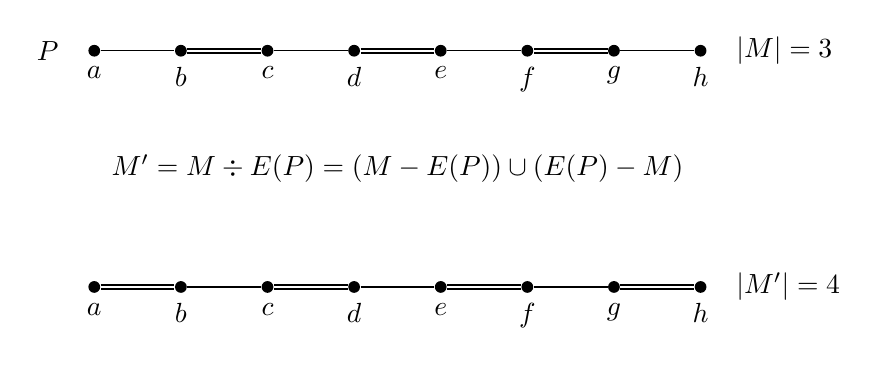
\begin{tikzpicture}[x=1.1cm]
		\begin{scope}
			\node[left] at (-0.3, 0) {$P$};
			\foreach \x/\l in {0/a, 1/b, 2/c, 3/d, 4/e, 5/f, 6/g, 7/h} {
					\node[circle, fill=black, inner sep=1.5pt, label=below:$\l$] (\l) at (\x, 0) {};
				}
			\draw (a) -- (b);
			\draw[double, thick] (b) -- (c);
			\draw (c) -- (d);
			\draw[double, thick] (d) -- (e);
			\draw (e) -- (f);
			\draw[double, thick] (f) -- (g);
			\draw (g) -- (h);
			\node[right] at (7.3, 0) {$|M|=3$};
		\end{scope}

		\begin{scope}[yshift=-1.5cm]
			\node at (3.5, 0) {$M' = M \div E(P) = (M - E(P)) \cup (E(P) - M)$};
		\end{scope}

		\begin{scope}[yshift=-3cm]
			\foreach \x/\l in {0/a, 1/b, 2/c, 3/d, 4/e, 5/f, 6/g, 7/h} {
					\node[circle, fill=black, inner sep=1.5pt, label=below:$\l$] (\l) at (\x, 0) {};
				}
			\draw[double, thick] (a) -- (b);
			\draw (b) -- (c);
			\draw[double, thick] (c) -- (d);
			\draw (d) -- (e);
			\draw[double, thick] (e) -- (f);
			\draw (f) -- (g);
			\draw[double, thick] (g) -- (h);
			\node[right] at (7.3, 0) {$|M'|=4$};
		\end{scope}
	\end{tikzpicture}
\end{azfigure}
Możemy użyć ścieżki powiększającej i różnicy symetrycznej do zwiększenia liczności skojarzenia.

\begin{obowiazkowy}
	\begin{theorem}[Berge'a]
		Niech $G=(V,E)$ -- graf, $M$ -- skojarzenie w $G$. \\
		$M$ jest najliczniejszym skojarzeniem w $G \iff$ nie istnieje ścieżka powiększająca względem $M$.
	\end{theorem}

	\begin{proof} ~
		\begin{itemize}
			\item[$\implies$]
			      Przypuśćmy, że istnieje ścieżka powiększająca $P$ względem $M$. \\
			      Wtedy $M' = M \div E(P)$ jest skojarzeniem i $|M'| > |M|$, więc $M$ nie jest skojarzeniem najliczniejszym.
			\item[$\impliedby$]
			      Przypuśćmy, że $M$ nie jest najliczniejszym skojarzeniem w $G$. \\
			      Niech $M'$ będzie skojarzeniem takim, że $|M'| > |M|$. \\
			      Niech $H$ będzie podgrafem $G$ indukowanym przez $M' \div M$, czyli $H = (V(G), M' \div M)$. \\
			      $M, M'$ to skojarzenia, więc stopień wierzchołka $d_H(v) \le 2$ dla każdego $v \in V(G)$.

			      Każda składowa $H$ jest ścieżką lub cyklem. \\
			      $M, M'$ to skojarzenia, więc nie ma cykli nieparzystych w $H$. \\
			      Każda składowa $H$ jest ścieżką lub cyklem parzystym. \\
			      Skoro $|M'| > |M|$, to istnieje składowa $H$, która jest ścieżką zawierającą więcej krawędzi z $M'$ niż z $M$, więc ta ścieżka zaczyna się i kończy krawędzią z $M'$. Ta ścieżka jest ścieżką powiększającą względem $M$. \qedhere
		\end{itemize}
	\end{proof}
\end{obowiazkowy}
